%!TEX root = thesis.tex

\chapter{Analyse}
\label{chapter-analyse}

Dieses Kapitel beschreibt alle für die Arbeit notwendigen Grundlagen.

\section{Datenquellen}
\label{section:daten}

\section{Benutzeranalyse}
\label{section:benutzer}

\section{Aufgabenanalyse}
\label{section:aufgaben}

\section{Kontextanalyse}
\label{section:kontext}

\section{Analyse des aktuellen Stands}
\label{section:iststand}

\section{Formalisierte Anforderungen}
\label{section:anforderung}

Im Folgenden werden systematisch formalisierte Anforderungen präsentiert, welche die Ergebnisse der Analysen abschließend zusammenfassen.
Es werden zunächst die Visionen und Ziele (\ref{section:visionziel}) definiert, des Weiteren werden
die Rahmenbedingungen (\ref{section:rahmen}) und der Kontext des Systems
(\ref{section:kontextueberblick}) dargestellt. Darauf aufbauend wird eine funktionale Anforderung
erstellt (\ref{section:funktionale}). Abschließen werden die Qualitätsanforderungen formuliert
(\ref{section:qualität}).


\subsection*{Vision und Ziele}
\label{section:visionziel}
Zunächst sollten die Visionen und Ziele des Systems konkretisiert werden, an denen sich die
Anforderungen auf Zielgerichtetheit überprüfen lassen \cite{balzert2009}. Diese setzen sich aus der
Analyse der Benutzenden sowie Aufgaben und des Kontextes zusammen. Im ersten Schritt werden die
Visionen für die Zukunft realitätsnah festgelegt.



\begin{center}
     \renewcommand{\arraystretch}{1.5}
    \begin{tabular}{p{0.1\textwidth}p{0.8\textwidth}}
    \hline
            \textbf{/V10/} & Erstellende des Status sind in der Lage, effizient zentrale
            Informationen darzustellen. \\
            \textbf{/V20/}  & Betrachtende sind besser dazu in der Lage, Erstellende zu
            kontaktieren, als aktuell.\\
    \hline
    \end{tabular}
\end{center}

Basierend auf diese Visionen lassen sich die Ziele formulieren, welche die Visionen
operationalisieren. Diese folgen dabei den standardisierten Regeln zur Formulierung von Zielen
\cite{pohl_requirements_2008}.


\begin{center}
     \renewcommand{\arraystretch}{1.5}
    \begin{tabular}{p{0.1\textwidth}p{0.8\textwidth}}
    \hline
            \textbf{/Z10/} & Betrachtende des Systems erhalten zielgerichtete und aktuelle
            Informationen zum Verbleib der aufgesuchten Person. \\
            \textbf{/Z20/} & Erstellende verwenden ein gebrauchstaugliches, niedrigschwelliges Interface zum Erstellen von Informationen\\
            \textbf{/Z30/} & Erstellende sind jederzeit in der Lage, ihre Informationen zu ändern.\\
            \textbf{/Z40/} & Erstellende sind überall in der Lage, ihre Informationen zu ändern.\\
            \textbf{/Z50/} & Der Status ist durch Erstellende leicht und unkompliziert veränderbar.\\
    \hline
    \end{tabular}
\end{center}

\subsection*{Rahmenbedingungen}
\label{section:rahmen}
Die Randbedingungen legen organisatorische und technische Restriktionen für das System oder den
Entwicklungsprozess fest \cite{balzert2009}. Die Bedingungen wurden aus dem Lastenheft und der
Benutzer- und Kontextanalyse abgeleitet.

\begin{center}
    \renewcommand{\arraystretch}{1.5}
    \begin{tabular}{p{0.1\textwidth}p{0.8\textwidth}}
    \hline
            \textbf{/R10/} & Das System ist eine Web-Anwendung.\\
            \textbf{/R20/} & Die Zielgruppe sind Mitarbeitende des IMIS und Studierende.\\
            \textbf{/R30/} & Die Zielgruppe teilt sich in zwei Nutzergruppen: die Erstellenden und
            Betrachtenden des Systems. Die Definitionen der Nutzergruppen sind in Kapitel (\ref{section:benutzer})
            zu finden.\\
            \textbf{/R40/} & Das System wird von Erstellenden sowohl im mobilen als auch im Arbeitskontext genutzt ().\\
            \textbf{/R50/} & Die eingesetzte Software auf der Zielmaschine ist clientseitig ein
            Webbrowser. Die marktführenden Webbrowser müssen unterstützt werden: Chrome, Firefox,
            Safari \cite{noauthor_browser_nodate}.\\
    \hline
    \end{tabular}
\end{center}

\subsection*{Kontext und Überblick}
\label{section:kontextueberblick}
Ein System ist in einer technischen Umgebung eingebettet \cite{balzert2009}. Es wurde im Folgenden Bezug auf das aktuelle Vorgehen und die Schnittstellen des System genommen.

\begin{center}
    \renewcommand{\arraystretch}{1.5}
    \begin{tabular}{p{0.1\textwidth}p{0.8\textwidth}}
    \hline
            \textbf{/K10/} & Das aktuelle Vorgehen umfasst Klebezettel an den Türen der Mitarbeitenden.\\
            \textbf{/K20/} & Es existiert eine Schnittstelle zum Back-End des Labormanagementsystems.\\
            \textbf{/K30/} & Es existiert ein digitaler Kalender, auf den die Mitarbeitenden Zugriff haben, in dem geblockte Zeiten einzelner Personen angezeigt werden.\\
    \hline
    \end{tabular}
\end{center}

\subsection*{Funktionale Anforderungen}
\label{section:funktionale}
Im Folgenden werden die Kernfunktionalitäten des Systems aufgeführt \cite{balzert2009}.
Diese ergeben sich aus der Aufgabenanalyse (section:aufgaben). Um die Anforderungen mit einer eindeutigen Semantik zu formulieren, wurde eine Anforderungsschablone (\ref{fig:schablone}) verwendet, um natürlichsprachliche Anforderungen zu definieren \cite{balzert2009}.

\begin{figure}[h]
        \centering
        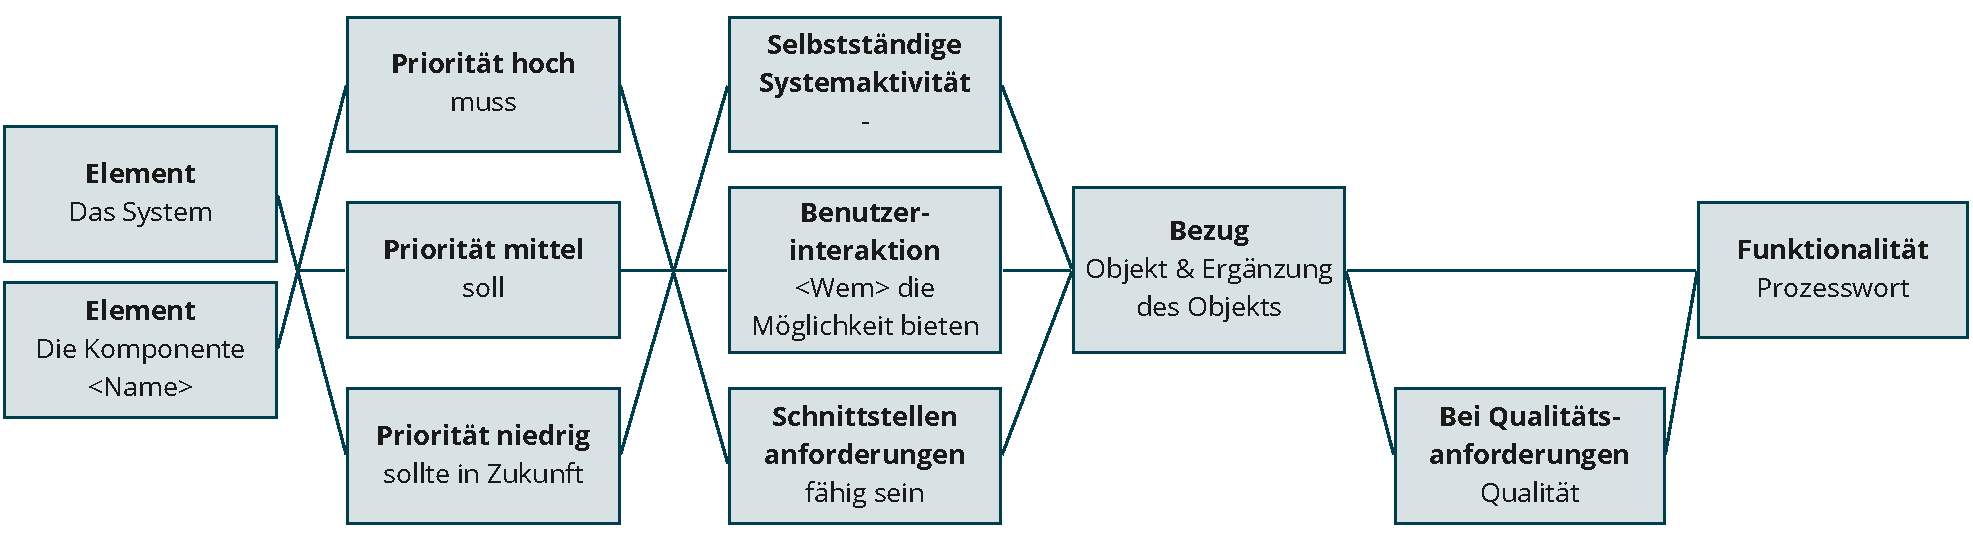
\includegraphics[scale=0.45]{Bilder/anforderungsschablone.pdf}
        \label{fig:schablone}
    \caption[Anforderungsschablone]{Anforderungsschablone \cite{balzert2009}}
\end{figure}

\begin{center}
    \renewcommand{\arraystretch}{1.5}
    \begin{tabular}{p{0.1\textwidth}p{0.8\textwidth}}
    \hline
            \textbf{/F10/} & Das System \textit{muss} Erstellenden die Möglichkeit bieten, Informationen jederzeit einzutragen (A).\\
            \textbf{/F20/} & Das System \textit{muss} Erstellenden die Möglichkeit bieten, Status wiederzuverwenden.\\
            \textbf{/F30/} & Das System \textit{muss} Erstellenden die Möglichkeit bieten, ein Profil zu erstellen (A).\\
            \textbf{/F40/} & Das System \textit{muss} Betrachtenden relevante Informationen anzeigen, welche vom Erstellenden hinterlassen werden sollen (A).\\
            \textbf{/F50/} & Das System \textit{muss} Erstellenden die Möglichkeit geben, den alleinigen Zugriff auf die eigenen Daten zu haben.\\
            \textbf{/F60/} & Das System \textit{soll} Erstellenden die Möglichkeit bieten, individuelle und personalisierte Inhalte zu visualisieren (A).\\
            \textbf{/F70/} & Das System \textit{soll} daran erinnern, die Informationen zu aktualisieren (A).\\
            \textbf{/F80/} & Das System \textit{soll} Erstellenden die Möglichkeit bieten, sich eine Vorschau ihres aktuell angezeigten Türschilds anzuschauen.\\
            \textbf{/F90/} & Das System \textit{sollte in Zukunft} die Möglichkeit bieten, per Schalter bedienbar zu sein.\\
            \textbf{/F100/} & Das System \textit{sollte in Zukunft} Betrachtenden die Möglichkeit bieten, Informationen zu hinterlassen (A).\\
            \textbf{/F110/} & Das System \textit{sollte in Zukunft} den angezeigten Status automatisch aus den Daten des digitalen Kalenders ermitteln können.\\
    \hline
    \end{tabular}
\end{center}


\subsection*{Qualitätsanforderungen}
\label{section:qualität}
Im letzten Schritt werden die nicht-funktionalen Anforderungen festgelegt, welche die qualitativen oder quantitativen Eigenschaften eines Systems darstellen \cite{balzert2009}. Auch hier wird, falls möglich, die Anforderungsschablone aus \ref{fig:schablone} verwendet.

\begin{center}
    \renewcommand{\arraystretch}{1.5}
    \begin{tabular}{p{0.1\textwidth}p{0.8\textwidth}}
    \hline
            \textbf{/Q10/} & Das System \textit{muss} den Grundsätzen der DIN EN ISO
            9241-110:2019-09 (Ergonomie der Mensch-System-Interaktion - Teil 110:
            Interaktionsprinzipien) folgen (\textit{DIN EN ISO 9241-110}, 2019).\\
            \textbf{/Q20/} & Das System \textit{muss} die definierten Nutzungsklassen aus Kapitel
            section:benutzer (Sonderrolle) unterscheiden und die dazugehörigen Zugriffsrechte
            sicherstellen.\\
            \textbf{/Q30/} & Das System \textit{soll} modular strukturiert sein, damit Inhalte und Funktionalitäten effizient eingebunden werden können und das System einfach erweiterbar ist.\\
            \textbf{/Q40/} & Das System \textit{soll} beim Zugriff über das Internet eine gesicherte Übertragung (bspw. HTTPS) ermöglichen.\\
            \textbf{/Q50/} & Das System \textit{soll} alle Benutzerinteraktionen in unter fünf Sekunden ausführen.\\
    \hline
    \end{tabular}
\end{center}
